%% bondgraph_example.tex
%% Copyright (c) 2010, Jean-Francois Dupuis
%
% This work may be distributed and/or modified under the
% conditions of the LaTeX Project Public License, either version 1.3
% of this license or (at your option) any later version.
% The latest version of this license is in
%   http://www.latex-project.org/lppl.txt
% and version 1.3 or later is part of all distributions of LaTeX
% version 2005/12/01 or later.
%
% This work has the LPPL maintenance status `maintained'.
% 
% The Current Maintainer of this work is Jean-Francois Dupuis.
%
% This work consists of the files bondgraph.sty, bondgraph_arrows.tex 
% and bondgraph_example.tex.

\documentclass{article}
\usepackage[x11names, rgb]{xcolor}
\usepackage[utf8]{inputenc}
\usepackage{bondgraph}

\begin{document}

\begin{figure}
	\centering
	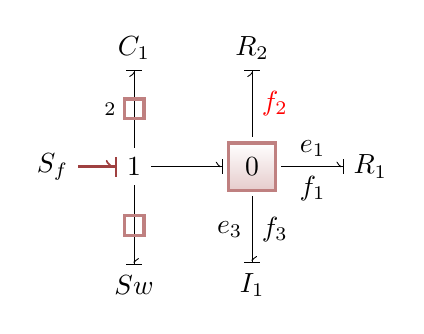
\begin{tikzpicture}
		[node distance=1.5cm]
		\bgComponentNoBond{S}{$S_f$}		
		\bgComponent{}{J11}{1}{right=0.5cm of}{S}{newelement,inbonde}
		\bgComponent{nodemodpoint}{J01}{0}{right of=}{J11}{inbonde}
		\bgComponentWithBondMarkupTagged{}{C1}{$C_1$}{above of=}{J11}{inbonde}{bondmodpoint}{2}
		\bgComponentWithBondLabel{}{R1}{$R_1$}{right of=}{J01}{inbonde}{}{$e_1$}{$f_1$}
		\bgComponentWithBondLabel{}{R2}{$R_2$}{above of=}{J01}{inbonde}{color=red}{}{$f_2$}
		\bgComponentWithBondLabel{}{I1}{$I_1$}{below of=}{J01}{inbonde}{}{$e_3$}{$f_3$}
		\bgComponentWithBondMarkup{}{Sw}{$Sw$}{below of=}{J11}{inbonde}{bondmodpoint}
		%\bgComponent{}{Sw}{$Sw$}{below of}{J11}{outbondf}
	\end{tikzpicture}
	\caption{Simplified bond graph definition.}
\end{figure}

\begin{figure}
\centering
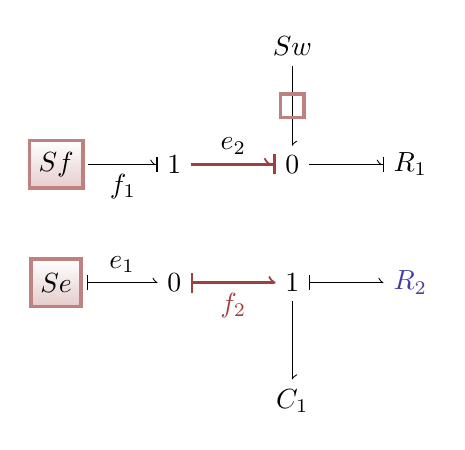
\begin{tikzpicture}
[
	node distance=1.5cm,
	mynewelement/.style={
		color=blue!50!black!75,
		thick
	},
	mybondmodpoint/.style={
	% The shape:
	rectangle,
	% The size:
	minimum size=3mm,
	% The border:
	very thick,
	draw=red!50!black!50, % 50% red and 50% black, and that mixed with 50% white
	% Seperation
	outer sep=2pt
	}
]
		
	\node [nodemodpoint] (S) {$Sf$};
	\node (J11) [right of=S]{1}
	edge [inbonde]  node [below]{$f_{1}$} (S);
	\node (J01) [right of=J11] {0}
	edge [newelement,inbonde]  node  [color=black] [above]{$e_{2}$} (J11);
	\node (R1) [right of=J01] {$R_1$}
	edge [inbonde]  (J01);
	\node (Sw) [above of=J01] {$Sw$}
	edge [outbond]  node [mybondmodpoint] {} (J01);
	
	
	\node [nodemodpoint] (S2) [below of=S]{$Se$};
	\node (J02) [right of=S2]{0}
	edge [inbondf]  node [above]{$e_{1}$} (S2);
	\node (J12) [right of=J02]{1}
	edge [newelement,inbondf]  node [below]{$f_{2}$} (J02);
	\node [mynewelement] (R2) [right of=J12]{$R_2$}
	edge [inbondf]  (J12);
	\node (C1) [below of=J12] {$C_1$}
	edge [inbond]  (J12);
\end{tikzpicture}

\caption{Bond graph example.}

\end{figure}
\end{document}
